\documentclass[tikz,border=5pt]{standalone}
\usepackage{luatexja}
\usepackage[hiragino-pron]{luatexja-preset}
\usepackage{amsmath,amssymb}
\usepackage{pgfplots}
\pgfplotsset{compat=1.18}
\usetikzlibrary{arrows.meta,calc,decorations.markings,patterns,positioning}

% Common styles
\tikzset{
  axis/.style={-{Stealth[length=6pt]}, thick},
  curve/.style={thick, red},
  dashed curve/.style={thick, dashed, blue},
  dot/.style={circle, fill, inner sep=1.5pt},
  open dot/.style={circle, draw, fill=white, inner sep=1.5pt},
}

\begin{document}
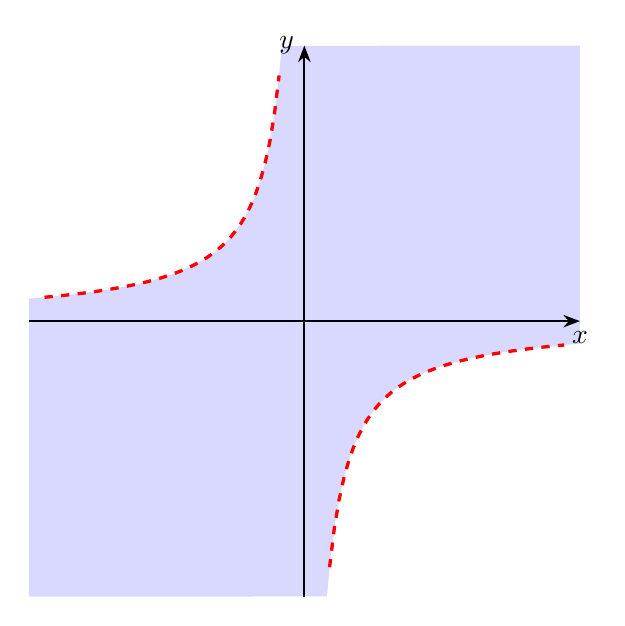
\begin{tikzpicture}
  % Upper fill: Q2 below curve + Q1 (plot is first element to avoid moveto bug)
  \fill[blue, opacity=0.15]
    plot[domain=-3.5:{-1/3.5}, samples=60] (\x, {-1/\x})
    -- (3.5, 3.5) -- (3.5, 0) -- (-3.5, 0) -- cycle;

  % Lower fill: Q4 above curve + all of Q3 (plot is first element)
  \fill[blue, opacity=0.15]
    plot[domain=3.5:{1/3.5}, samples=60] (\x, {-1/\x})
    -- (-3.5, -3.5) -- (-3.5, 0) -- (3.5, 0) -- cycle;

  % Axes
  \draw[axis] (-3.5,0) -- (3.5,0) node[below] {$x$};
  \draw[axis] (0,-3.5) -- (0,3.5) node[left] {$y$};

  % Hyperbola xy = -1 (red dashed)
  \draw[red, dashed, very thick, domain=-3.3:-0.32, samples=50] plot (\x, {-1/\x});
  \draw[red, dashed, very thick, domain=0.32:3.3, samples=50] plot (\x, {-1/\x});
\end{tikzpicture}
\end{document}
